\documentclass[12pt,twoside,a4paper]{article}
\usepackage[utf8]{inputenc}
\usepackage[T1]{fontenc}
\usepackage{amsfonts}
\usepackage{amssymb}
\usepackage{amsmath}
\usepackage[pdftex]{graphicx}


\title{Java Project Course: Minesweeper}
\author{Madeleine Ekblom}

\begin{document}

\maketitle
\section{Documentation, part 1}

\subsubsection*{Subject: Minesweeper}
A one-player-game where you try to find all the mines without denotating any of them. The nxm-large gameboard 
is filled with sqaures, which are ordered in n rows and m columns. Under some squares mines are hidden and by 
help of the given numbers on the open squares you are supposed to mark the mines. The faster the mines are found, 
the better it is. The level on the game depends on how big the gameboard is and how many mines that are hidden.  \\

\underline{Actors: Computer, player} \\ 

\underline{Computer's function:} \\
	- Genarates a nxm-large gameboard with x mines \\
	\ 	- The places for mines are chosen randomly \\
	- Marks the non-mine-squares with numbers depending on how many mines are found around the square. \\
	  \ - If the square doesn't have any mines around, it will be empty (instead of having a zero) \\
	- Creates a high-score list, and updates it  \\

\underline{Player's function:} \\
	- Opens the squares and depending on what kind of square it is, marks the mines with flags \\
	- Tries to find the mines as fast as possible \\ 
	- Wins if all the mines are found, else the computer wins \\

\section{Documentation, part 2}

\subsection{Class diagram, week 3}
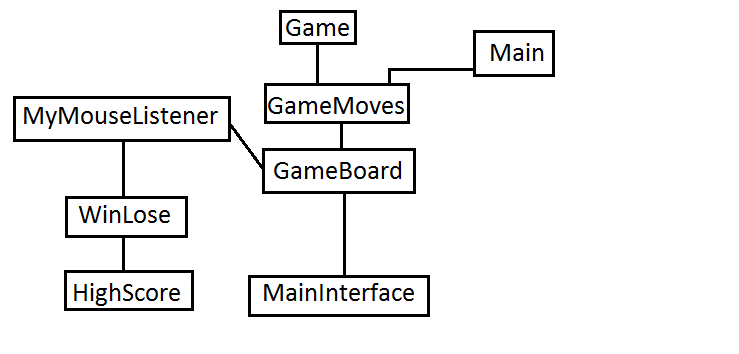
\includegraphics{classdiagram.png}



\end{document}